\documentclass[aspectratio=169, table, 12pt]{beamer}

\usepackage{colortbl}
\usepackage{xcolor}
\usepackage{tabularx}
\usepackage{tikz}
\usetikzlibrary{arrows.meta, positioning, calc, fit, shapes.geometric}

\makeatletter
\def\input@path{{../theme/}}
\makeatother
\graphicspath{{../theme/}{../../figures/}}
\usetheme{Pradita}

\definecolor{praditagreen}{RGB}{37, 113, 71}

% One color per agent, the same as on the monitor page and in the draw.io diagram.
\definecolor{alicecolor}{RGB}{138, 63, 184}
\definecolor{bobcolor}{RGB}{44, 100, 214}
\definecolor{charliecolor}{RGB}{176, 112, 12}
\definecolor{davidcolor}{RGB}{15, 138, 138}
\definecolor{erincolor}{RGB}{45, 138, 87}
\definecolor{frankcolor}{RGB}{194, 65, 59}

% The two series of the human effort chart, checked for color vision deficiency.
\definecolor{beforecolor}{HTML}{2A78D6}
\definecolor{aftercolor}{HTML}{257147}

% The theme draws table rules in white. Black rules keep tables readable.
\arrayrulecolor{black}
\setlength{\arrayrulewidth}{0.5pt}

% A left-aligned X column, so narrow columns do not stretch the spaces between words.
\newcolumntype{Y}{>{\raggedright\arraybackslash}X}

\title{\Huge Agentic SDLC\\ \vspace{10pt} \LARGE Six Agents, One User Story}
\subtitle{Concepts, Organization, and a Case Study}
\author{\textbf{Alfa Yohannis}}

\begin{document}

\frame{\titlepage}

\begin{frame}
  \frametitle{Contents}
  \vspace{14pt}
  \begin{columns}[t]
    \column{0.5\textwidth}
    {\small\tableofcontents[sections={1-4}]}

    \column{0.5\textwidth}
    {\small\tableofcontents[sections={5-8}]}
  \end{columns}
\end{frame}

\begin{frame}{\hfill}
  \centering
  \Huge{\textbf{What happens when every role\\on the team is held by an agent?}}
\end{frame}

% ---------------------------------------------------------------------------
\section{Goals}

\begin{frame}{\hfill}
  \centering
  \Huge{\textbf{Goals}}
\end{frame}

\begin{frame}{{\Large Learning Goals}}
  \vspace{12pt}
  \begin{itemize}
    \item Explain the agentic SDLC cycle and its test-first variant: the
          phases agents carry out, the gates people keep, and the feedback
          loops.
    \item Describe how a team of agents is organized and coordinated: roles,
          ownership, layers of context, and orchestration or choreography.
    \item Reason about autonomy and control: what agents may do on their own,
          and what needs a person.
  \end{itemize}
\end{frame}

% ---------------------------------------------------------------------------
\section{Agentic SDLC in General}

\begin{frame}{\hfill}
  \centering
  \Huge{\textbf{Agentic SDLC in General}}
\end{frame}

\begin{frame}{{\Large From SDLC to Agentic SDLC}}
  \vspace{10pt}
  \begin{itemize}
    \item The software development life cycle (SDLC) splits building software
          into phases: specification, design, build, test, deployment, and
          operation.
    \item In an agentic SDLC the phases stay, but AI agents do the work inside
          them. They draft user stories, propose an architecture, write code
          and tests, and run the pipeline.
    \item People set the goal, the constraints, and the risk at the start, and
          they hold two decision gates in the middle of the cycle.
  \end{itemize}
  \vspace{6pt}
  {\small The gates keep the responsibility for what is built and released
  with people, however fast the agents work.}
\end{frame}

\begin{frame}{{\Large The Agentic SDLC Cycle}}
  \vspace{2pt}
  \centering
  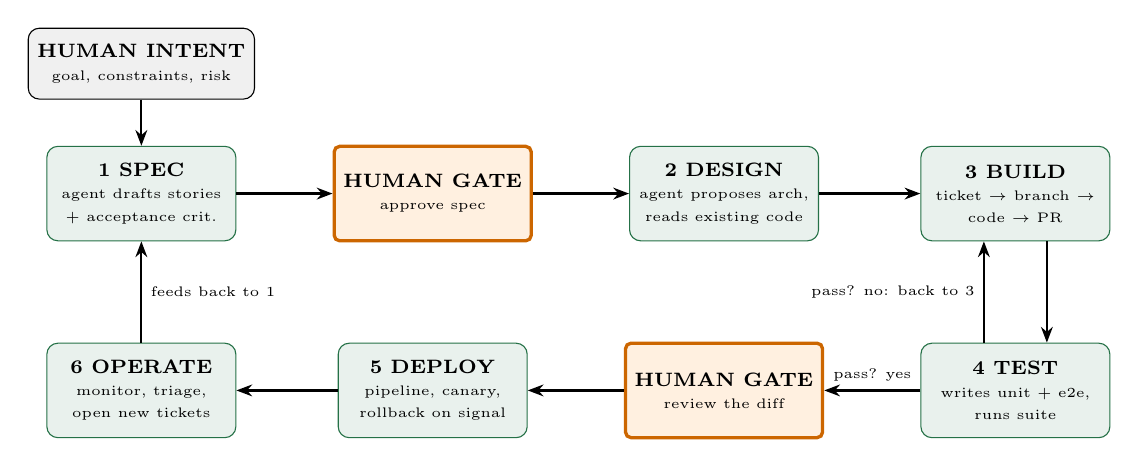
\begin{tikzpicture}[
    phase/.style={draw=praditagreen, fill=praditagreen!10, rounded corners,
                  minimum width=2.4cm, minimum height=1.2cm, align=center,
                  font=\scriptsize},
    gate/.style={draw=orange!80!black, very thick, fill=orange!12,
                 rounded corners=2pt, minimum width=2.4cm,
                 minimum height=1.2cm, align=center, font=\scriptsize},
    intent/.style={draw, fill=gray!12, rounded corners, minimum width=2.4cm,
                   minimum height=0.9cm, align=center, font=\scriptsize},
    arrow/.style={-{Stealth[length=2mm]}, thick},
    note/.style={font=\tiny, fill=white, inner sep=1pt}
  ]
    \node[intent] (intent) at (0,2.55) {\textbf{HUMAN INTENT}\\{\tiny goal, constraints, risk}};

    \node[phase] (spec) at (0,0.9) {\textbf{1 SPEC}\\{\tiny agent drafts stories}\\{\tiny + acceptance crit.}};
    \node[gate] (g1) at (3.7,0.9) {\textbf{HUMAN GATE}\\{\tiny approve spec}};
    \node[phase] (design) at (7.4,0.9) {\textbf{2 DESIGN}\\{\tiny agent proposes arch,}\\{\tiny reads existing code}};
    \node[phase] (build) at (11.1,0.9) {\textbf{3 BUILD}\\{\tiny ticket $\rightarrow$ branch $\rightarrow$}\\{\tiny code $\rightarrow$ PR}};

    \node[phase] (test) at (11.1,-1.6) {\textbf{4 TEST}\\{\tiny writes unit + e2e,}\\{\tiny runs suite}};
    \node[gate] (g2) at (7.4,-1.6) {\textbf{HUMAN GATE}\\{\tiny review the diff}};
    \node[phase] (deploy) at (3.7,-1.6) {\textbf{5 DEPLOY}\\{\tiny pipeline, canary,}\\{\tiny rollback on signal}};
    \node[phase] (operate) at (0,-1.6) {\textbf{6 OPERATE}\\{\tiny monitor, triage,}\\{\tiny open new tickets}};

    \draw[arrow] (intent) -- (spec);
    \draw[arrow] (spec) -- (g1);
    \draw[arrow] (g1) -- (design);
    \draw[arrow] (design) -- (build);
    \draw[arrow] ([xshift=4mm]build.south) -- ([xshift=4mm]test.north);
    \draw[arrow] ([xshift=-4mm]test.north) -- node[note, left=2pt] {pass? no: back to 3} ([xshift=-4mm]build.south);
    \draw[arrow] (test) -- node[note, above=2pt] {pass? yes} (g2);
    \draw[arrow] (g2) -- (deploy);
    \draw[arrow] (deploy) -- (operate);
    \draw[arrow] (operate) -- node[note, right=2pt] {feeds back to 1} (spec);
  \end{tikzpicture}

  \vspace{6pt}
  {\footnotesize Green boxes are agent work. Orange boxes are human decisions.}
\end{frame}

\begin{frame}{{\Large Human Gates}}
  \vspace{10pt}
  \begin{itemize}
    \item The first gate approves the specification. Before any design or
          code exists, a person checks that the user stories and acceptance
          criteria say what they meant. A misunderstanding is cheapest to fix
          here.
    \item The second gate reviews the diff. Before release, a person reads the
          changes that passed the tests, because passing tests only prove the
          behavior they test.
    \item Between the two gates, agents may loop on their own: write code, run
          the tests, and fix what fails without waiting for anyone.
  \end{itemize}
\end{frame}

\begin{frame}{{\Large Two Feedback Loops}}
  \vspace{10pt}
  \begin{itemize}
    \item Inner loop: when a test fails, the work goes back to BUILD. Agents
          run this loop themselves, as often as it takes.
    \item Outer loop: OPERATE watches the running application and triages
          the problems it finds, which means sorting them by impact and
          urgency, setting duplicates and noise aside, and deciding who
          handles each one. The result is new tickets that go back into
          SPEC.
  \end{itemize}
  \vspace{8pt}
  {\small The inner loop keeps the code in line with the specification. The
  outer loop keeps the specification in line with what happens in
  production.}
\end{frame}

\begin{frame}{{\Large Who Does What}}
  \vspace{4pt}
  \centering
  {\footnotesize
  \begin{tabularx}{\textwidth}{lYY}
    \hline
    \textbf{Phase} & \textbf{Agent} & \textbf{Human} \\
    \hline
    SPEC & drafts user stories and acceptance criteria & states the goal, constraints, and risk, then approves the specification \\
    \hline
    DESIGN & proposes an architecture after reading the existing code & - \\
    \hline
    BUILD & ticket, branch, code, then a pull request & - \\
    \hline
    TEST & writes unit and end-to-end tests and runs the suite & - \\
    \hline
    DEPLOY & pipeline, canary release, rollback on a signal & reviews the diff before release \\
    \hline
    OPERATE & monitors, triages problems by impact and urgency, opens new tickets & - \\
    \hline
  \end{tabularx}}
\end{frame}

\begin{frame}{{\Large Where Human Effort Goes}}
  \vspace{2pt}
  \begin{columns}[c]
    \column{0.58\textwidth}
    \centering
    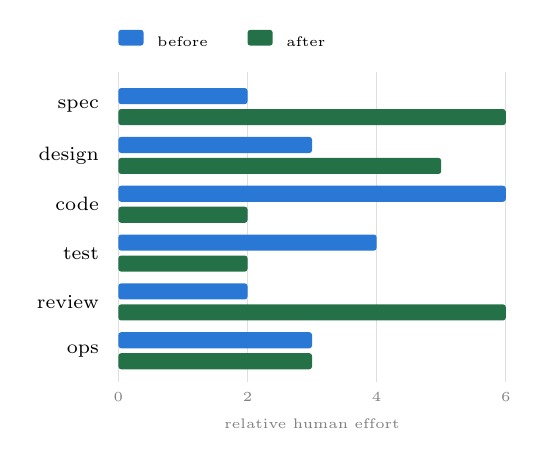
\begin{tikzpicture}[x=0.82cm, y=0.62cm, font=\scriptsize]
      % Legend, above the plot.
      \fill[beforecolor, rounded corners=1pt] (0,6.75) rectangle ++(0.32cm,0.2cm);
      \node[anchor=west, font=\tiny] at (0.45,6.83) {before};
      \fill[aftercolor, rounded corners=1pt] (2.0,6.75) rectangle ++(0.32cm,0.2cm);
      \node[anchor=west, font=\tiny] at (2.45,6.83) {after};

      % Recessive grid and axis.
      \foreach \v in {0,2,4,6} {
        \draw[gray!25] (\v,-0.15) -- (\v,6.2);
        \node[gray, font=\tiny, below] at (\v,-0.15) {\v};
      }
      \node[gray, font=\tiny] at (3,-1.0) {relative human effort};

      % One row per phase: the before bar above the after bar.
      \foreach \phase/\before/\after [count=\i from 0] in
          {spec/2/6, design/3/5, code/6/2, test/4/2, review/2/6, ops/3/3} {
        \pgfmathsetmacro{\y}{5.5-\i}
        \node[anchor=east] at (-0.15,\y) {\phase};
        \fill[beforecolor, rounded corners=1pt] (0,\y+0.05) rectangle (\before,\y+0.38);
        \fill[aftercolor, rounded corners=1pt] (0,\y-0.38) rectangle (\after,\y-0.05);
      }
    \end{tikzpicture}

    \column{0.42\textwidth}
    \small
    \begin{itemize}
      \item Less effort on code (from 6 to 2) and tests (from 4 to 2).
      \item More effort on the specification (from 2 to 6), design (from 3
            to 5), and review (from 2 to 6).
      \item Operations stays at 3.
    \end{itemize}
    \vspace{4pt}
    {\footnotesize People spend their time saying what to build and checking
    what was built. Agents do most of the building in between.}
  \end{columns}
\end{frame}

% ---------------------------------------------------------------------------
\section{Organizing an Agent Team}

\begin{frame}{\hfill}
  \centering
  \Huge{\textbf{Organizing an Agent Team}}
\end{frame}

\begin{frame}{{\Large One Orchestrator, Many Agents}}
  \vspace{2pt}
  \begin{columns}[c]
    \column{0.6\textwidth}
    \centering
    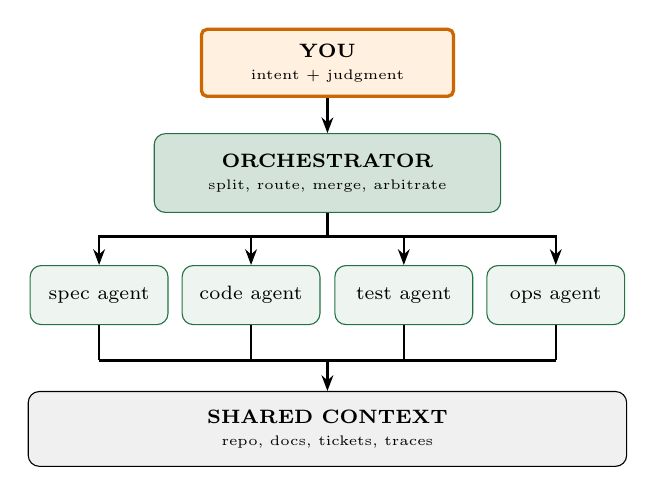
\begin{tikzpicture}[
      person/.style={draw=orange!80!black, very thick, fill=orange!12,
                     rounded corners=2pt, minimum width=3.2cm,
                     minimum height=0.85cm, align=center, font=\scriptsize},
      orchestrator/.style={draw=praditagreen, fill=praditagreen!20,
                           rounded corners, minimum width=4.4cm,
                           minimum height=1.0cm, align=center, font=\scriptsize},
      agent/.style={draw=praditagreen, fill=praditagreen!8, rounded corners,
                    minimum width=1.75cm, minimum height=0.75cm, align=center,
                    font=\scriptsize},
      context/.style={draw, fill=gray!12, rounded corners, minimum width=7.6cm,
                      minimum height=0.95cm, align=center, font=\scriptsize},
      arrow/.style={-{Stealth[length=2mm]}, thick}
    ]
      \node[person] (you) at (0,3.4) {\textbf{YOU}\\{\tiny intent + judgment}};
      \node[orchestrator] (orch) at (0,2.0) {\textbf{ORCHESTRATOR}\\{\tiny split, route, merge, arbitrate}};
      \node[agent] (spec) at (-2.9,0.45) {spec agent};
      \node[agent] (code) at (-0.97,0.45) {code agent};
      \node[agent] (test) at (0.97,0.45) {test agent};
      \node[agent] (ops) at (2.9,0.45) {ops agent};
      \node[context] (ctx) at (0,-1.25) {\textbf{SHARED CONTEXT}\\{\tiny repo, docs, tickets, traces}};

      \draw[arrow] (you) -- (orch);
      \foreach \a in {spec, code, test, ops} {
        \draw[arrow] (orch.south) -- ++(0,-0.3) -| (\a.north);
        \draw[thick] (\a.south) -- (\a.south |- 0,-0.38);
      }
      \draw[thick] (-2.9,-0.38) -- (2.9,-0.38);
      \draw[arrow] (0,-0.38) -- (ctx.north);
    \end{tikzpicture}

    \column{0.4\textwidth}
    \small
    \begin{itemize}
      \item The orchestrator splits a goal into tasks, routes each task to an
            agent, merges the results, and decides when agents disagree.
      \item Every agent works from the same shared context: the repository,
            the docs, the tickets, and the traces of earlier runs.
      \item The person talks to the orchestrator and keeps the final judgment.
    \end{itemize}
  \end{columns}
\end{frame}

\begin{frame}{{\Large Orchestration and Choreography}}
  \vspace{10pt}
  \centering
  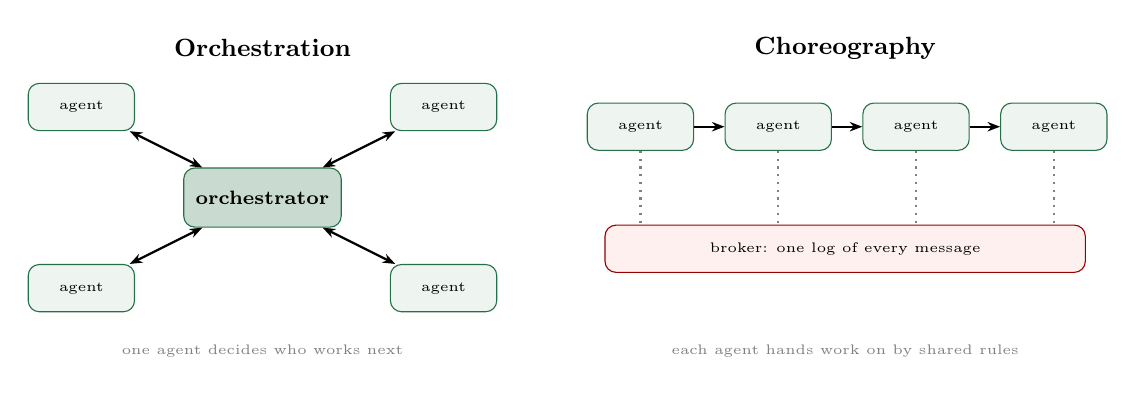
\begin{tikzpicture}[
    agent/.style={draw=praditagreen, fill=praditagreen!8, rounded corners,
                  minimum width=1.35cm, minimum height=0.6cm, align=center,
                  font=\tiny},
    hub/.style={draw=praditagreen, fill=praditagreen!25, rounded corners,
                minimum width=2.0cm, minimum height=0.75cm, align=center,
                font=\scriptsize\bfseries},
    log/.style={draw=red!60!black, fill=red!6, rounded corners,
                minimum height=0.6cm, align=center, font=\tiny},
    arrow/.style={-{Stealth[length=1.6mm]}, thick},
    both/.style={{Stealth[length=1.6mm]}-{Stealth[length=1.6mm]}, thick}
  ]
    % Orchestration: hub and spokes.
    \node[font=\small\bfseries] at (3,2.9) {Orchestration};
    \node[hub] (hub) at (3,1.0) {orchestrator};
    \node[agent] (o1) at (0.7,2.15) {agent};
    \node[agent] (o2) at (5.3,2.15) {agent};
    \node[agent] (o3) at (0.7,-0.15) {agent};
    \node[agent] (o4) at (5.3,-0.15) {agent};
    \foreach \a in {o1, o2, o3, o4} { \draw[both] (hub) -- (\a); }
    \node[font=\tiny, gray] at (3,-0.95) {one agent decides who works next};

    % Choreography: a chain of handoffs over a shared log.
    \node[font=\small\bfseries] at (10.4,2.9) {Choreography};
    \node[agent] (c1) at (7.8,1.9) {agent};
    \node[agent] (c2) at (9.55,1.9) {agent};
    \node[agent] (c3) at (11.3,1.9) {agent};
    \node[agent] (c4) at (13.05,1.9) {agent};
    \draw[arrow] (c1) -- (c2);
    \draw[arrow] (c2) -- (c3);
    \draw[arrow] (c3) -- (c4);
    \node[log, minimum width=6.1cm] (log) at (10.4,0.35) {broker: one log of every message};
    \foreach \a in {c1, c2, c3, c4} { \draw[dotted, thick, gray] (\a.south) -- (\a.south |- log.north); }
    \node[font=\tiny, gray] at (10.4,-0.95) {each agent hands work on by shared rules};
  \end{tikzpicture}

  \vspace{10pt}
  {\small An orchestrator gives one point of control and one point of failure.
  Choreography spreads the decisions over the agents, so the shared rules and
  the message log have to carry the coordination. This case study uses
  choreography.}
\end{frame}

\begin{frame}{{\Large Choosing a Coordination Pattern}}
  \vspace{4pt}
  \centering
  {\footnotesize
  \begin{tabularx}{\textwidth}{lYY}
    \hline
    & \textbf{Orchestration} & \textbf{Choreography} \\
    \hline
    Who decides the next step & the orchestrator & each agent, from the team's rules \\
    \hline
    Control and failure & one central point & spread over the agents \\
    \hline
    Adding an agent & change the orchestrator & add the agent and update the rules \\
    \hline
    Where to see what happened & the orchestrator's records & the message log \\
    \hline
    Suits & work that must be split and rebalanced as it goes & a workflow that is known in advance \\
    \hline
  \end{tabularx}}
\end{frame}

\begin{frame}{{\Large Roles and Ownership}}
  \vspace{10pt}
  \begin{itemize}
    \item Each agent has one role and owns a set of artifacts. Alice owns the
          specification, Bob the tests, Charlie the database, Frank the back
          end, David the front end, and Erin the documentation.
    \item Every agent may read everything, but it changes only what it owns.
          A change to another artifact goes to its owner as a message.
    \item Ownership keeps two agents from editing the same file at once, and
          it gives a clear answer to the question of who is responsible.
  \end{itemize}
  \vspace{6pt}
  {\small This is code ownership, as human teams practise it, applied to
  agents.}
\end{frame}

\begin{frame}{{\Large Layers of Context}}
  \vspace{8pt}
  \centering
  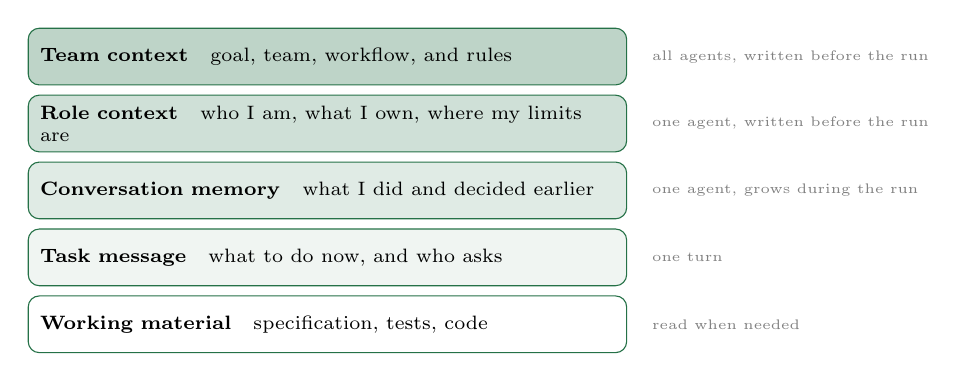
\begin{tikzpicture}[
    layer/.style={draw=praditagreen, rounded corners, minimum width=7.6cm,
                  minimum height=0.72cm, align=left, font=\scriptsize,
                  text width=7.3cm},
    scope/.style={font=\tiny, gray, anchor=west, align=left}
  ]
    \node[layer, fill=praditagreen!30] (team) at (0,2.8) {\textbf{Team context}\quad goal, team, workflow, and rules};
    \node[layer, fill=praditagreen!22] (role) at (0,1.95) {\textbf{Role context}\quad who I am, what I own, where my limits are};
    \node[layer, fill=praditagreen!14] (memory) at (0,1.1) {\textbf{Conversation memory}\quad what I did and decided earlier};
    \node[layer, fill=praditagreen!7] (task) at (0,0.25) {\textbf{Task message}\quad what to do now, and who asks};
    \node[layer, fill=white] (work) at (0,-0.6) {\textbf{Working material}\quad specification, tests, code};

    \node[scope] at (4.0,2.8) {all agents, written before the run};
    \node[scope] at (4.0,1.95) {one agent, written before the run};
    \node[scope] at (4.0,1.1) {one agent, grows during the run};
    \node[scope] at (4.0,0.25) {one turn};
    \node[scope] at (4.0,-0.6) {read when needed};
  \end{tikzpicture}

  \vspace{10pt}
  {\small An agent knows only what these layers tell it. Anything the team
  depends on has to be written into one of them.}
\end{frame}

% ---------------------------------------------------------------------------
\section{A Test-First Process}

\begin{frame}{\hfill}
  \centering
  \Huge{\textbf{A Test-First Process}}
\end{frame}

\begin{frame}{{\Large A Test-First Variant of the Cycle}}
  \vspace{0pt}
  \centering
  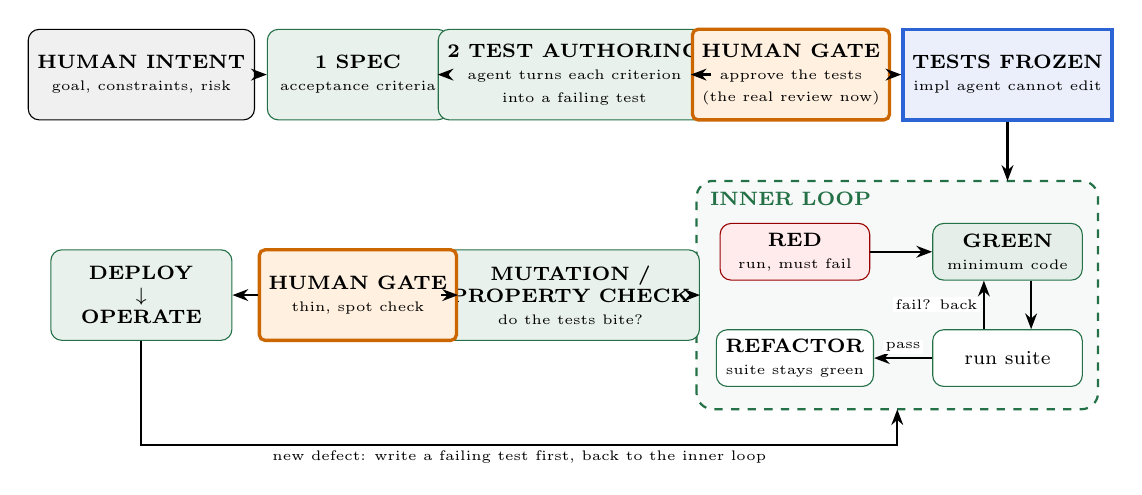
\begin{tikzpicture}[
    phase/.style={draw=praditagreen, fill=praditagreen!10, rounded corners,
                  minimum width=2.3cm, minimum height=1.15cm, align=center,
                  font=\scriptsize},
    gate/.style={draw=orange!80!black, very thick, fill=orange!12,
                 rounded corners=2pt, minimum width=2.3cm,
                 minimum height=1.15cm, align=center, font=\scriptsize},
    frozen/.style={draw=bobcolor, very thick, fill=bobcolor!10,
                   minimum width=2.3cm, minimum height=1.15cm, align=center,
                   font=\scriptsize},
    intent/.style={draw, fill=gray!12, rounded corners, minimum width=2.3cm,
                   minimum height=1.15cm, align=center, font=\scriptsize},
    loopstep/.style={draw=praditagreen, fill=white, rounded corners,
                 minimum width=1.9cm, minimum height=0.72cm, align=center,
                 font=\scriptsize},
    arrow/.style={-{Stealth[length=2mm]}, thick},
    note/.style={font=\tiny, fill=white, inner sep=1pt}
  ]
    % Row 1, left to right.
    \node[intent] (intent) at (0,2.3) {\textbf{HUMAN INTENT}\\{\tiny goal, constraints, risk}};
    \node[phase] (spec) at (2.75,2.3) {\textbf{1 SPEC}\\{\tiny acceptance criteria}};
    \node[phase] (author) at (5.5,2.3) {\textbf{2 TEST AUTHORING}\\{\tiny agent turns each criterion}\\{\tiny into a failing test}};
    \node[gate] (g1) at (8.25,2.3) {\textbf{HUMAN GATE}\\{\tiny approve the tests}\\{\tiny (the real review now)}};
    \node[frozen] (frozen) at (11.0,2.3) {\textbf{TESTS FROZEN}\\{\tiny impl agent cannot edit}};

    % The inner loop, under the right end of row 1.
    \draw[praditagreen, thick, dashed, rounded corners=6pt, fill=praditagreen!4]
      (7.05,-1.95) rectangle (12.15,0.95);
    \node[anchor=north west, font=\scriptsize\bfseries, text=praditagreen] at (7.1,0.93) {INNER LOOP};
    \node[loopstep, fill=red!8, draw=red!60!black] (red) at (8.3,0.05) {\textbf{RED}\\{\tiny run, must fail}};
    \node[loopstep, fill=praditagreen!12] (green) at (11.0,0.05) {\textbf{GREEN}\\{\tiny minimum code}};
    \node[loopstep] (suite) at (11.0,-1.3) {run suite};
    \node[loopstep] (refactor) at (8.3,-1.3) {\textbf{REFACTOR}\\{\tiny suite stays green}};

    % Row 2, right to left.
    \node[phase, minimum width=2.25cm] (mutation) at (5.45,-0.5) {\textbf{MUTATION /}\\\textbf{PROPERTY CHECK}\\{\tiny do the tests bite?}};
    \node[gate] (g2) at (2.75,-0.5) {\textbf{HUMAN GATE}\\{\tiny thin, spot check}};
    \node[phase] (ops) at (0,-0.5) {\textbf{DEPLOY}\\$\downarrow$\\\textbf{OPERATE}};

    \draw[arrow] (intent) -- (spec);
    \draw[arrow] (spec) -- (author);
    \draw[arrow] (author) -- (g1);
    \draw[arrow] (g1) -- (frozen);
    \draw[arrow] (frozen) -- (11.0,0.95);

    \draw[arrow] (red) -- (green);
    \draw[arrow] ([xshift=3mm]green.south) -- ([xshift=3mm]suite.north);
    \draw[arrow] ([xshift=-3mm]suite.north) -- node[note, left=1pt] {fail? back} ([xshift=-3mm]green.south);
    \draw[arrow] (suite) -- node[note, above=1pt] {pass} (refactor);

    \draw[arrow] (7.05,-0.5) -- (mutation);
    \draw[arrow] (mutation) -- (g2);
    \draw[arrow] (g2) -- (ops);
    \draw[arrow] (ops.south) -- (0,-2.4) -- node[note, below=1pt] {new defect: write a failing test first, back to the inner loop} (9.6,-2.4) -- (9.6,-1.95);
  \end{tikzpicture}
\end{frame}

\begin{frame}{{\Large What Changes in the Test-First Variant}}
  \vspace{6pt}
  \begin{itemize}
    \item The human review moves to the tests. Once a person approves them,
          the tests are the specification the code has to meet.
    \item The tests are frozen, so the implementing agent cannot make a
          failing test pass by editing it.
    \item In the inner loop the agent goes red, green, refactor: the new test
          fails, the smallest change makes it pass, and refactoring keeps the
          suite green.
    \item A mutation or property check tests the tests: change the code on
          purpose, and some test should fail.
    \item The last human gate shrinks to a spot check. A new defect starts as
          a failing test.
  \end{itemize}
\end{frame}

\begin{frame}{{\Large Tests as Contracts Between Agents}}
  \vspace{10pt}
  \begin{itemize}
    \item When the tests are written first, they fix the interfaces before
          any code exists: the data functions, the login API, and the elements
          on the page.
    \item With the interfaces fixed, the database, back-end, and front-end
          agents can work at the same time without waiting for each other.
    \item A failing test tells its owner exactly what is missing. A dispute
          about a test goes back to the agent who owns the tests.
  \end{itemize}
  \vspace{6pt}
  {\small In one run, Frank noticed that a test contradicted the
  specification and asked Bob to change it. Bob agreed and fixed the test
  before Frank went on.}
\end{frame}

\begin{frame}{{\Large Handoffs and Definitions of Done}}
  \vspace{10pt}
  \begin{itemize}
    \item A handoff is an explicit message: what is ready, where it is, and
          what the receiver needs to know.
    \item Each role has its own definition of done. The specification is done
          when it can be tested. The tests are done when they fail for the
          right reason. The code is done when its tests pass. The docs are
          done when they match the code.
    \item Erin starts only after three handoffs have arrived, which makes her
          step a join point in the process.
  \end{itemize}
  \vspace{6pt}
  {\small A reply arrives as a new message, so no agent sits blocked while it
  waits for an answer.}
\end{frame}

% ---------------------------------------------------------------------------
\section{The Case Study}

\begin{frame}{\hfill}
  \centering
  \Huge{\textbf{The Case Study}}
\end{frame}

\begin{frame}{{\Large The User Story: A Login Page}}
  \vspace{10pt}
  \begin{itemize}
    \item The user logs in with an email address, and its format is checked.
    \item The password has at least three words and at least two spaces, for
          example ``green apple house''.
    \item A button shows and hides the password.
    \item Errors come with messages a user understands.
    \item Three failed attempts lock the login for five seconds, and the page
          tells the user to wait.
  \end{itemize}
  \vspace{8pt}
  {\small Written by a person acting as product owner. Everything after this
  point is done by the agents.}
\end{frame}

\begin{frame}{{\Large Six Roles}}
  \vspace{4pt}
  \centering
  {\footnotesize
  \begin{tabularx}{\textwidth}{clYY}
    \hline
    \textbf{Agent} & \textbf{Name} & \textbf{Role} & \textbf{Owns} \\
    \hline
    A & \textcolor{alicecolor}{\textbf{Alice}} & Requirements analyst & the specification \\
    \hline
    B & \textcolor{bobcolor}{\textbf{Bob}} & Test engineer, tests first & the tests and the test contract \\
    \hline
    C & \textcolor{charliecolor}{\textbf{Charlie}} & Database developer & the database layer \\
    \hline
    D & \textcolor{davidcolor}{\textbf{David}} & Front-end developer & the login page \\
    \hline
    E & \textcolor{erincolor}{\textbf{Erin}} & Technical writer & the documentation \\
    \hline
    F & \textcolor{frankcolor}{\textbf{Frank}} & Back-end developer & the login API and the lockout rule \\
    \hline
  \end{tabularx}}

  \vspace{8pt}
  {\small The source code of the whole setup is at
  \href{https://github.com/alfa-yohannis/agentic-sdlc}{\texttt{github.com/alfa-yohannis/agentic-sdlc}}.}
\end{frame}

\begin{frame}[t]{{\Large Workflow}}
  \vspace{26pt}
  \centering
  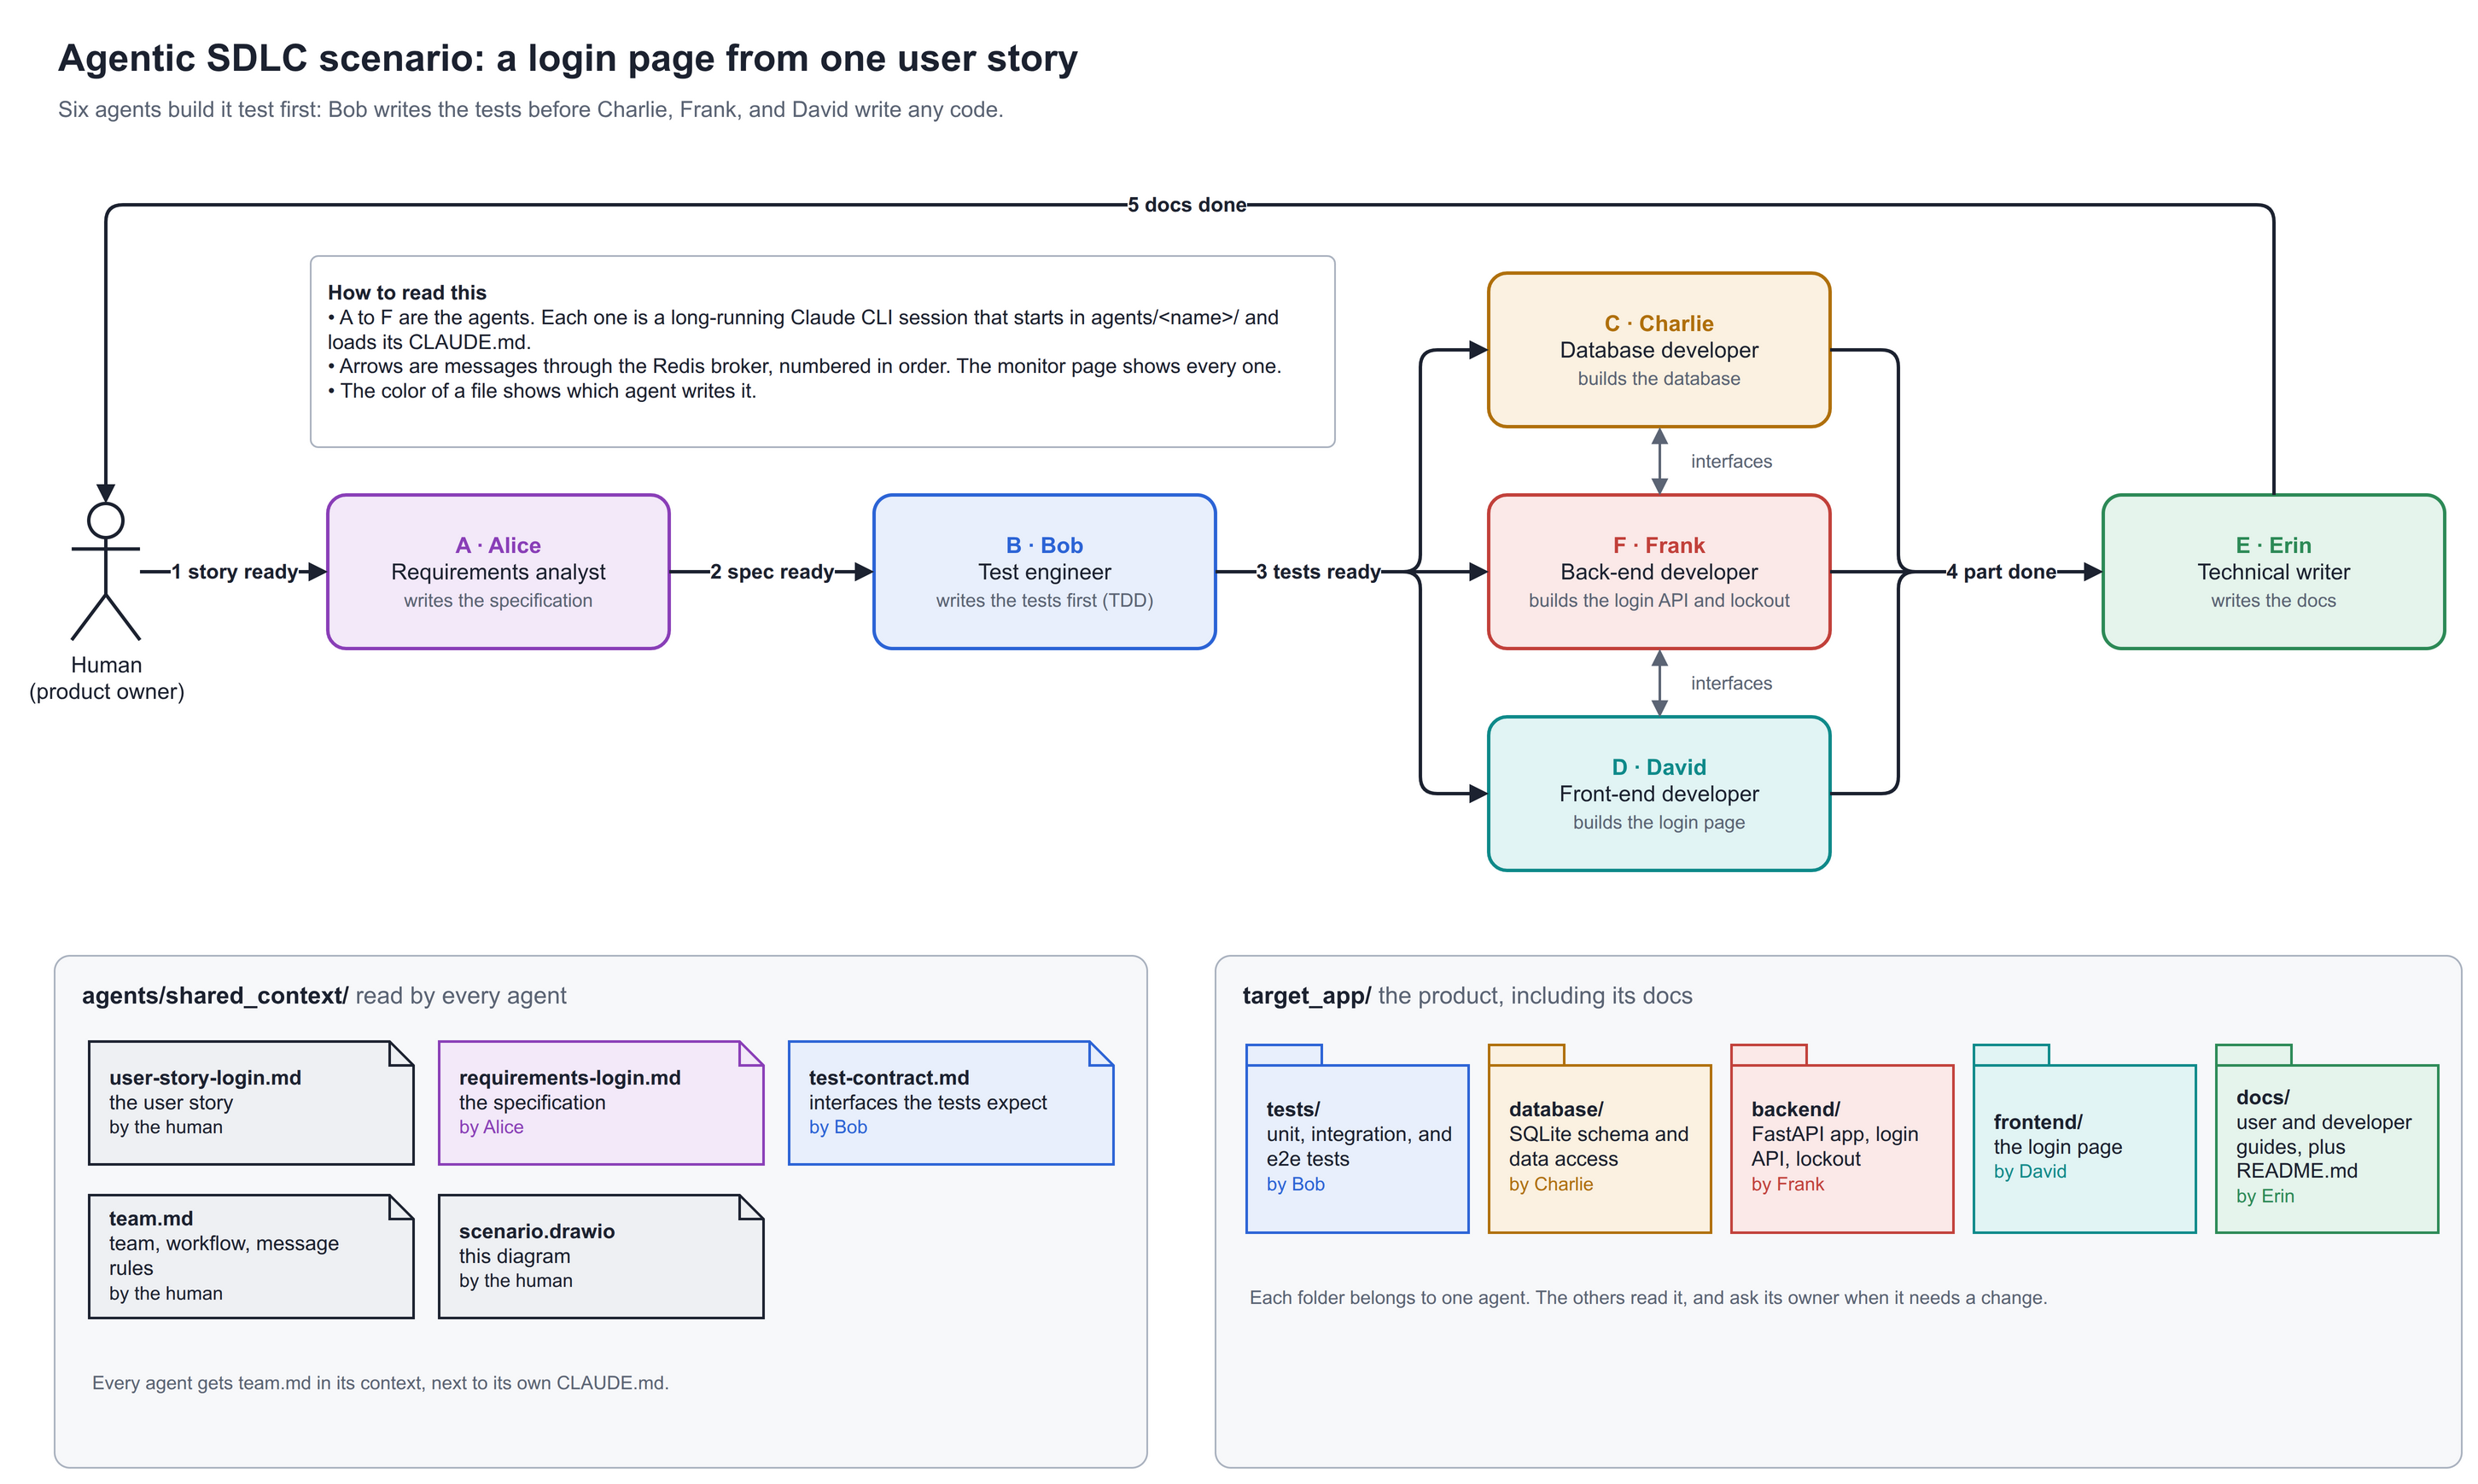
\includegraphics[width=\textwidth, height=0.74\textheight, keepaspectratio]{scenario.png}
\end{frame}

\begin{frame}{{\Large What the First Run Produced}}
  \vspace{4pt}
  \centering
  {\footnotesize
  \begin{tabularx}{\textwidth}{lY}
    \hline
    \textbf{Artifact} & \textbf{Contents} \\
    \hline
    Specification & 2 validation rules, 25 functional and 17 non-functional requirements, 23 acceptance criteria, and 6 open questions for the product owner \\
    \hline
    Tests & 138 test functions: 49 unit, 35 integration, and 54 end-to-end \\
    \hline
    Test contract & the interfaces the tests expect from the database, the back end, and the front end \\
    \hline
    Code & database layer, back end, and login page, written against the contract \\
    \hline
  \end{tabularx}}

  \vspace{8pt}
  {\small Alice turned vague phrases such as ``a simple error message'' into
  testable rules and wrote down her assumptions. What she could not decide
  went to the human as questions.}
\end{frame}

\begin{frame}{{\Large This Case Study in the Cycle}}
  \vspace{0pt}
  \centering
  {\scriptsize
  \begin{tabularx}{\textwidth}{lY}
    \hline
    \textbf{Part} & \textbf{In this case study} \\
    \hline
    SPEC & the human writes the user story, Alice writes the specification and its acceptance criteria \\
    \hline
    Approve spec & not in place yet: Alice hands the specification straight to Bob \\
    \hline
    DESIGN & partly: the team context fixes the tech stack, and the test contract fixes the interfaces \\
    \hline
    Test authoring & Bob turns the acceptance criteria into tests before any code exists \\
    \hline
    Tests frozen & by instruction only: the developers are told not to edit the tests \\
    \hline
    BUILD & Charlie, Frank, and David build their parts at the same time, without branches or pull requests \\
    \hline
    Orchestrator & none: the agents hand work to each other through the broker \\
    \hline
    Documentation & Erin, after the tests pass \\
    \hline
    Mutation check, deploy, operate & outside this case study \\
    \hline
  \end{tabularx}}

  \vspace{4pt}
  {\footnotesize The missing parts are the next steps, for example making
  Alice wait for human approval before she hands the specification to Bob.}
\end{frame}

% ---------------------------------------------------------------------------
\section{Architecture}

\begin{frame}{\hfill}
  \centering
  \Huge{\textbf{Architecture}}
\end{frame}

\begin{frame}{{\Large A Conceptual Architecture}}
  \vspace{4pt}
  \centering
  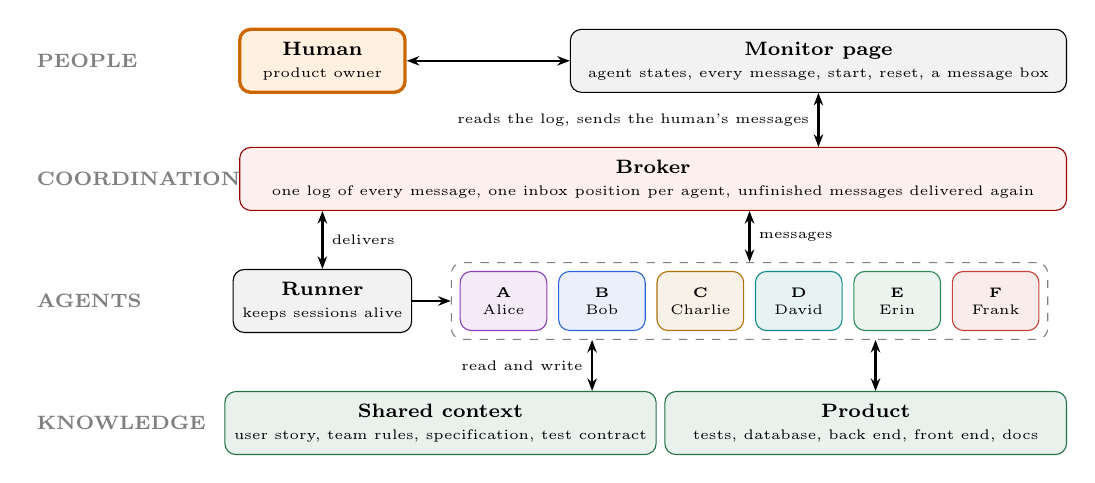
\begin{tikzpicture}[
    layername/.style={font=\scriptsize\bfseries, gray, anchor=west},
    part/.style={draw, rounded corners, minimum height=0.8cm, align=center,
                 font=\scriptsize},
    person/.style={part, draw=orange!80!black, very thick, fill=orange!12},
    agent/.style={part, minimum width=1.1cm, minimum height=0.75cm, font=\tiny},
    arrow/.style={{Stealth[length=1.6mm]}-{Stealth[length=1.6mm]}, thick},
    note/.style={font=\tiny, fill=white, inner sep=1pt}
  ]
    \node[layername] at (0,2.5) {PEOPLE};
    \node[layername] at (0,1.0) {COORDINATION};
    \node[layername] at (0,-0.55) {AGENTS};
    \node[layername] at (0,-2.1) {KNOWLEDGE};

    \node[person, minimum width=2.1cm] (human) at (3.75,2.5) {\textbf{Human}\\{\tiny product owner}};
    \node[part, fill=gray!10, minimum width=6.3cm] (monitor) at (10.05,2.5)
      {\textbf{Monitor page}\\{\tiny agent states, every message, start, reset, a message box}};

    \node[part, draw=red!60!black, fill=red!6, minimum width=10.5cm] (broker) at (7.95,1.0)
      {\textbf{Broker}\\{\tiny one log of every message, one inbox position per agent, unfinished messages delivered again}};

    \node[part, fill=gray!10, minimum width=2.1cm] (runner) at (3.75,-0.55) {\textbf{Runner}\\{\tiny keeps sessions alive}};
    \foreach \name/\letter/\c [count=\i from 0] in
        {Alice/A/alicecolor, Bob/B/bobcolor, Charlie/C/charliecolor,
         David/D/davidcolor, Erin/E/erincolor, Frank/F/frankcolor} {
      \node[agent, draw=\c, fill=\c!10] (a\i) at (6.05+\i*1.25,-0.55) {\textbf{\letter}\\\name};
    }
    \node[draw, dashed, gray, rounded corners, fit=(a0) (a5), inner sep=3pt] (agents) {};

    \node[part, fill=praditagreen!10, draw=praditagreen, minimum width=5.1cm] (shared) at (5.25,-2.1)
      {\textbf{Shared context}\\{\tiny user story, team rules, specification, test contract}};
    \node[part, fill=praditagreen!10, draw=praditagreen, minimum width=5.1cm] (product) at (10.65,-2.1)
      {\textbf{Product}\\{\tiny tests, database, back end, front end, docs}};

    \draw[arrow] (human) -- (monitor);
    \draw[arrow] (monitor.south) -- node[note, left=2pt] {reads the log, sends the human's messages} (monitor.south |- broker.north);
    \draw[arrow] (runner.north) -- node[note, right=2pt] {delivers} (runner.north |- broker.south);
    \draw[arrow] (agents.north) -- node[note, right=2pt] {messages} (agents.north |- broker.south);
    \draw[-{Stealth[length=1.6mm]}, thick] (runner) -- (agents);
    \draw[arrow] ([xshift=-20mm]agents.south) -- node[note, left=2pt] {read and write} ([xshift=-20mm]agents.south |- shared.north);
    \draw[arrow] ([xshift=16mm]agents.south) -- ([xshift=16mm]agents.south |- product.north);
  \end{tikzpicture}
\end{frame}

\begin{frame}{{\Large Components and Responsibilities}}
  \vspace{4pt}
  \centering
  {\footnotesize
  \begin{tabularx}{\textwidth}{lY}
    \hline
    \textbf{Component} & \textbf{Responsibility} \\
    \hline
    Monitor page & shows each agent's state and every message, starts and resets the team, lets the human message an agent \\
    \hline
    Broker & keeps one log of all messages, gives each agent its own position in the log, delivers again what was not finished \\
    \hline
    Runner & keeps one long-running session per agent, turns each message into a turn, restarts a session that dies \\
    \hline
    Agent session & holds one role, its context, and a conversation that continues from message to message \\
    \hline
    Shared context & the team's common knowledge: goal, rules, specification, contracts \\
    \hline
    Product & what the team builds: code, tests, documentation \\
    \hline
  \end{tabularx}}
\end{frame}

\begin{frame}{{\Large Three Messaging Patterns}}
  \vspace{6pt}
  \centering
  {\footnotesize
  \begin{tabularx}{\textwidth}{Ylll}
    \hline
    & \textbf{Broadcast} & \textbf{Queue} & \textbf{Log} \\
    \hline
    Messages are kept & no & until taken & yes \\
    \hline
    A recipient that is down & loses the message & gets it later & gets it later \\
    \hline
    History for observers & none & gone once taken & complete \\
    \hline
    Completion is confirmed & no & no & yes \\
    \hline
  \end{tabularx}}

  \vspace{8pt}
  {\small The team uses a log. One structure delivers messages to the agents
  and gives the monitor the complete history, and every agent keeps its own
  reading position in it.}
\end{frame}

\begin{frame}{{\Large One Log, One Position per Agent}}
  \vspace{14pt}
  \centering
  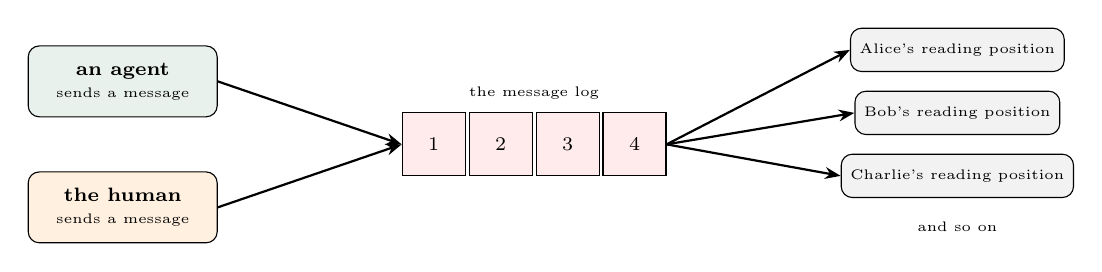
\begin{tikzpicture}[
    box/.style={draw, rounded corners, minimum height=0.9cm,
                minimum width=2.4cm, align=center, font=\scriptsize\bfseries},
    entry/.style={draw, fill=red!8, minimum height=0.8cm, minimum width=0.8cm,
                  font=\scriptsize},
    reader/.style={draw, rounded corners, fill=gray!10, minimum height=0.55cm,
                   minimum width=2.6cm, font=\tiny},
    arrow/.style={-{Stealth[length=2mm]}, thick}
  ]
    \node[box, fill=praditagreen!10] (agents) at (0,0.8) {an agent\\{\tiny\mdseries sends a message}};
    \node[box, fill=orange!12] (human) at (0,-0.8) {the human\\{\tiny\mdseries sends a message}};
    \foreach \i in {1,...,4} {
      \node[entry] (e\i) at (3.1+\i*0.85,0) {\i};
    }
    \node[font=\tiny, anchor=south] at ($(e2)!0.5!(e3)+(0,0.45)$) {the message log};
    \draw[arrow] (agents.east) -- (e1.west);
    \draw[arrow] (human.east) -- (e1.west);

    \node[reader] (g1) at (10.6,1.2) {Alice's reading position};
    \node[reader] (g2) at (10.6,0.4) {Bob's reading position};
    \node[reader] (g3) at (10.6,-0.4) {Charlie's reading position};
    \node[font=\tiny] at (10.6,-1.05) {and so on};
    \draw[arrow] (e4.east) -- (g1.west);
    \draw[arrow] (e4.east) -- (g2.west);
    \draw[arrow] (e4.east) -- (g3.west);
  \end{tikzpicture}

  \vspace{12pt}
  {\small Every message reaches every reading position, and each agent takes
  only the messages addressed to it. A message counts as handled once the
  agent's turn on it has ended, so an interrupted turn is delivered again.}
\end{frame}

\begin{frame}{{\Large Agents as Long-Running Sessions}}
  \vspace{10pt}
  \begin{itemize}
    \item Each agent is a session that stays alive between messages, so it
          remembers what it did and why.
    \item A message becomes a new turn in the same conversation. While it
          waits, the session costs nothing.
    \item When a session dies, it is restarted with its memory, and the
          unfinished message is delivered again.
  \end{itemize}
  \vspace{6pt}
  {\small The simpler alternative starts a fresh session for each task, which
  rereads its context and forgets everything in between.}
\end{frame}

\begin{frame}[t]{{\Large Watching the Team}}
  \vspace{30pt}
  \centering
  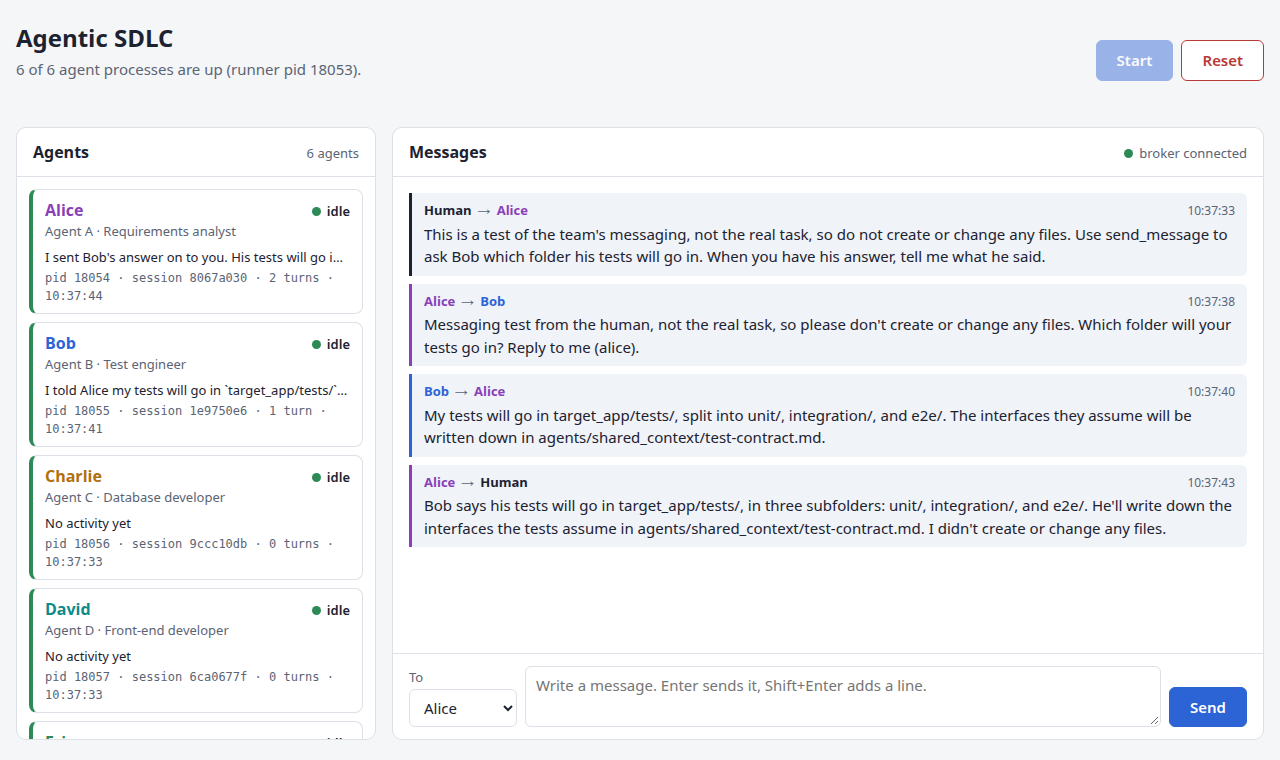
\includegraphics[width=\textwidth, height=0.6\textheight, keepaspectratio]{monitor.png}

  {\footnotesize Left: the agents and what each one is doing. Right: every
  message between them, including those to and from the human.}
\end{frame}

% ---------------------------------------------------------------------------
\begin{frame}{{\Large Granting Just Enough}}
  \vspace{10pt}
  \begin{itemize}
    \item The tester and the developers get one narrow capability: prepare the
          app's environment and run its tests.
    \item Alice only writes the specification, so she received nothing.
    \item Running tests means running code, so the agents belong on a machine
          you trust, or in a container.
  \end{itemize}
  \vspace{6pt}
  {\small Least privilege applies to agents as it does to people and
  services: grant per capability, and grant only what the role needs.}
\end{frame}

% ---------------------------------------------------------------------------
\section{Lessons and Open Questions}

\begin{frame}{\hfill}
  \centering
  \Huge{\textbf{Lessons and Open Questions}}
\end{frame}

\begin{frame}{{\Large Lessons from the Case Study}}
  \vspace{6pt}
  \begin{itemize}
    \item Context has to be explicit. An agent knows only what its context
          layers and its messages tell it.
    \item Tests written first work as contracts and let three agents build at
          the same time.
    \item A broker makes the collaboration visible, because every handoff and
          question can be read afterwards.
    \item Refusing by default turns a blocker into a question for a person.
    \item Agents follow the process they are given, so the human gates have to
          be designed in from the start.
  \end{itemize}
\end{frame}

\begin{frame}{{\Large Open Questions}}
  \vspace{6pt}
  \begin{itemize}
    \item Where should the human gates sit, and how much should each one
          check?
    \item How can tests be frozen by the system, and not only by
          instruction?
    \item When does an orchestrator help, and when is choreography enough?
    \item How do we know that the tests are strong enough, for example through
          mutation testing?
    \item How do the time and usage of an agent team compare with the same
          work done by people?
  \end{itemize}
\end{frame}

% ---------------------------------------------------------------------------
\section{Summary}

\begin{frame}{\hfill}
  \centering
  \Huge{\textbf{Summary}}
\end{frame}

\begin{frame}{{\Large Summary}}
  \vspace{6pt}
  \begin{itemize}
    \item An agentic SDLC keeps the SDLC phases. Agents do the work inside
          them, and people keep the intent and the gates.
    \item Human effort moves from writing code and tests to specifying and
          reviewing.
    \item An agent team needs roles, ownership, layered context, and a
          coordination pattern: an orchestrator, or choreography through a
          broker.
    \item A test-first process turns approved tests into the contract the code
          must meet, and lets agents build in parallel.
    \item Autonomy works inside boundaries: refuse by default, grant narrow
          capabilities, and keep every message visible.
  \end{itemize}
\end{frame}

\begin{frame}{\hfill}
  \centering
  {\Large\textbf{Source Code}}

  \vspace{12pt}
  {\Large\href{https://github.com/alfa-yohannis/agentic-sdlc}{\texttt{github.com/alfa-yohannis/agentic-sdlc}}}

  \vspace{12pt}
  {\small The agent team, the monitor page, the documentation, and these
  slides.}
\end{frame}

\end{document}
